\chapter[Lezione VI]{Lezione VI\newline\small{\emph{28/04/2011}}}
	\section{Strutture Dati}
		\subsection{Grafo}
		\label{subsec:grafo}
Un \emph{grafo} (figura~\ref{fig:grafo}) è un oggetto $G = (V, E)$ composto da \emph{vertici}\index{vertice} $v_n\in V$ e \emph{lati} $e_m\in E$. Si ha che:
\[
\begin{split}
&V=\{(x_1,y_1),\dots,(x_n,y_n)\} \\
&E\subseteq V\times V
\end{split}
\]
\begin{wrapfloat}{figure}{i}{0pt}{
	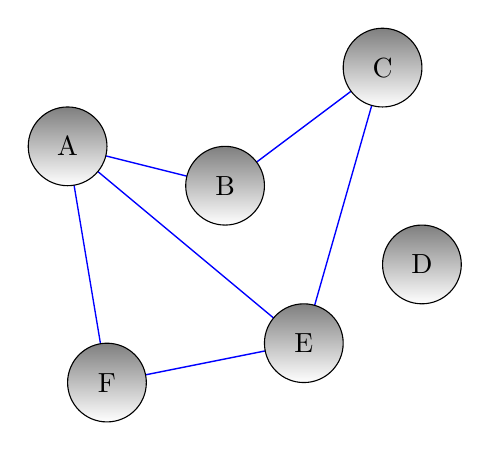
\begin{tikzpicture}
		\coordinate (A) at (0,4.5);
		\coordinate (B) at (2,4);
		\coordinate (C) at (4,5.5);
		\coordinate (D) at (4.5,3);
		\coordinate (E) at (3,2);
		\coordinate (F) at (0.5,1.5);
	
		\foreach \a/\b in {A/B, B/C, C/E, E/F, A/F, A/E}
			\draw [line width=0.5pt, color=blue] (\a) -- (\b);
	
		\foreach \n in {A,B,C,D,E,F} 
			\draw [] node [circle,draw,minimum size=1cm,top color=gray] at (\n) {\color{black}{\n}};
	\end{tikzpicture}
}
%	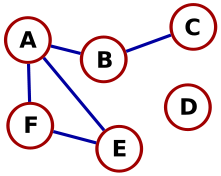
\includegraphics[width=0.5\columnwidth]{immagini/grafo}
	\caption{Esempio di grafo.}
	\label{fig:grafo}
\end{wrapfloat}
L'insieme dei lati è un sottoinsieme del prodotto cartesiano dei punti: ciascuno di essi è \emph{univocamente} determinato da una coppia di punti---se non è orientato.
Un lato, quindi, è un segmento non orientato completamente individuato da una coppia di punti.
Se consideriamo dei segmenti orientati, probabilmente, il grafo sarà una funzione di grandezze diverse.
Bisogna cioè aggiungere altre informazioni.

Supponiamo di avere segmenti non orientati e siano $v_1,v_2\in V$.
Per indicare un segmento che congiunga $v_1$ e $v_2$, le rappresentazioni $\overline{v_{1}v_{2}}$ e $\overline{v_{2}v_{1}}$ coincidono.
Nel caso di segmenti orientati, tuttavia, possiamo stabilire per convenzione che il primo punto sia l'origine del segmento, il verso sia indicato dal secondo punto e che la differenza tra i vertici permetta di stabilire il modulo del vettore.
Quindi, per un vettore orientato da $v_1$ a $v_2$ basterà scrivere $\overline{v_{1}v_{2}}$ oppure $\overrightarrow{v_{1}v_{2}}$.

		\subsection{Strutture}
		\label{subsec:record}
Si supponga di voler creare un programma che tenga traccia della carriera scolastica di alcuni studenti.
Innanzitutto, bisogna cercare di selezionare i dati essenziali ai fini del programma.
Si può immaginare lo studente come un ente univocamente determinato da tre variabili.
Si dichiarano, allora:\footnote{Si può anche dichiarare \lstinline!char n_matricola[6];! ma è molto più semplice che a rappresentare la matricola sia un numero (intero).}
\begin{lstlisting}
char nome[24];
int n_matricola;
int voti[6];
\end{lstlisting}
Queste variabili, tuttavia, sono ancora indipendenti tra di loro.
Dal momento che si riferiscono ad una stessa persona, sarebbe più utile poterle trattare come se fossero tutte ``legate''.
È\marginpar{Record} questo il concetto di \emph{record}\index{record}.
Un record permette di trattare più variabili non omogenee, come se fossero aggregate tra di loro.
\begin{lstlisting}[caption={[\em Struttura e variabili] {\em Definizione di una struttura e dichiarazione di variabili.}}, label={cod:struct}]
struct studente {
	char nome[24];
	int matricola, voti[6];
} maria, antonio;

int main ( int argc, char *argv[] ) {
	struct studente giuseppe, giovanni;
	£!\MyComment{\dots}!£
}
\end{lstlisting}
Nella fattispecie, il record \lstinline!studenti! contiene tre \emph{campi}\index{record!campo}.
Nel linguaggio \lang{C}, il record prende il nome di \emph{struttura}\index{struttura}.
La definizione delle strutture segue generalmente le prime direttive in cima al codice sorgente (\lstinline!#include <!\MyComment{header}\lstinline!>!) in modo che risulti ben visibile.
Si noti che dichiarare una struttura equivale, di fatto, a definire un nuovo tipo di variabile.

Nel codice~\vref{cod:struct} \lstinline!studente! è l'\emph{identificatore}\index{record!identificatore}, o \emph{tag}\index{record!tag}, della struttura.\footnote{Non è strettamente necessario introdurre la tag ma, per motivi di leggibilità, è fortemente consigliato.}
All'interno delle parentesi graffe (obbligatorie) si dichiarano le variabili che formeranno i campi della struttura.
\`E possibile dichiarare delle variabili di tipo \lstinline!struct studente! immediatamente dopo la definizione della struttura (come \lstinline!maria! e \lstinline!antonio! nel codice~\ref{cod:struct}).
Alternativamente, è consentito farlo in qualsiasi altra riga di codice, usando la sintassi descritta nel codice~\ref{cod:struct} per la dichiarazione di \lstinline!giuseppe! e \lstinline!giovanni!.


Il linguaggio \lang{C} consente\marginpar{\lstinline!typedef!} di assegnare un ``sinomimo'' a \lstinline!struct studente! tramite l'istruzione ``\lstinline!typedef tipo_1 tipo_2;!''\index{typedef@\texttt{typedef}}:
\begin{lstlisting}[caption={\em \lstinline!typedef! e assegnamenti.}, label={cod:strass}]
typedef struct studente Studente;

int main ( int argc, char *argv[] ) {
	Studente maria, antonio;

	maria.matricola = 73659;£!\label{assegnamento:1}!£
	maria.voti[2] = 27;£!\label{assegnamento:2}!£

	£!\MyComment{\dots}!£

}
\end{lstlisting}
In questo modo, si possono dichiarare delle variabili di tipo \lstinline!struct studente!, tramite il nuovo tipo \lstinline!Studente!.
Volendo richiamare (o assegnare un valore ad) un campo della struttura, la sintassi è riportata nelle righe~\ref{assegnamento:1} e~\ref{assegnamento:2} del codice~\ref{cod:strass}.
La regola è:
\begin{lstlisting}
£!\MyComment{nome}!£.£!\MyComment{campo}!£ = £!\MyComment{valore}!£;
\end{lstlisting}


Si tenga presente che, avendo dichiarato due record, \lstinline!a! e \lstinline!b!, è lecito operare un assegnamento nel modo usuale \lstinline!a = b!.
Tuttavia, non si possono confrontare due strutture con la scrittura ``\lstinline!a == b!'' ma bisogna confrontare le strutture campo per campo.

\begin{code}
\begin{minipage}{0.45\columnwidth}
	\begin{lstlisting}[caption={\em La direttiva \lstinline?\#define?.}, label={cod:def}]
#include <£!\MyComment{\dots}!£>
#define L 30

struct nome {
	char name[L];
};
	\end{lstlisting}
\end{minipage}	\hfill
\begin{minipage}{0.45\columnwidth}
	\begin{lstlisting}[caption={\em Punto e rettangolo.}, label={cod:ptrt}]
struct punto {
	double x;
	double y;
}
struct rettangolo {
	struct punto a_sx;
	struct punto b_dx;
}
	\end{lstlisting}
\end{minipage}

\end{code}
Spesso \marginpar{Direttiva \lstinline!#define!} può risultare conveniente specificare una direttiva\index{direttiva} \lstinline!#define!\index{define@\texttt{\#define}} all'inizio del codice sorgente come mostrato nel codice~\vref{cod:def}.\footnote{Le direttive \emph{non} sono istruzioni, quindi non bisogna concludere la riga con <<\lstinline!;!>>.}
Dopo aver specificato questa direttiva, il compilatore sostituirà il valore \num{30} ogni qualvolta incontrerà il carattere <<\lstinline!L!>>.
Il carattere deve essere una \emph{unità logica}, cioè, il compilatore non sostituirà il valore \num{30} a \lstinline!L! se esso è (ad esempio) all'interno di una parola.
Tale direttiva renderà il programma molto più facile da modificare.

Si supponga di voler creare una struttura che rappresenti un punto nello spazio bidimensionale.
Oltre alla rappresentazione vettoriale, è possibile utilizzare un record composto da due campi, come nel codice~\ref{cod:ptrt}.
Inoltre, poiché un rettangolo (parallelogramma retto) è univocamente individuato dagli estremi della sua diagonale, ci bastano due punti.



	\section{Stringhe}
In \lang{C} non esiste un tipo di variabile specifico per gestire le \emph{stringhe}.\footnote{In Informatica, una stringa è una sequenza di caratteri (ad esempio, una parola).}
Le stringhe vengono trattate come sequenze di caratteri.
Per memorizzarle, quindi, si renderà necessario dichiarare un array di caratteri.
In \lang{C}, ogni stringa termina con un carattere speciale detto \emph{terminatore}\index{terminatore} e rappresentato con  \lstinline!'\0'!.
Si noti che anch'esso occupa lo spazio di un carattere in memoria.

La\marginpar{La funzione \lstinline!strcpy()!} funzione \lstinline[mathescape]+strcpy( $\text{\MyComment{destinazione}}$, $\text{\MyComment{sorgente}}$ )+ copia una stringa da un array di caratteri \MyComment{sorgente}, specificato come secondo argomento reale, ad un altro array \MyComment{destinazione}, indicato dal primo parametro reale.
\begin{lstlisting}[caption={\em \lstinline!strcpy()! e \lstinline!scanf()!.}, label={cod:strcpy}]
struct studente {
	char nome[24];
	int matricola, voti[6];
} maria, antonio;

int main ( int argc, char *argv[] ) {
	strcpy(maria.nome, "Maria");
	scanf("%s", &antonio.nome);
	
	£!\MyComment{\dots}!£

}
\end{lstlisting}
Si può sfruttare tale funzione anche per effettuare un assegnamento, come nel codice~\ref{cod:strcpy}.
In alternativa, è possibile usare la funzione \lstinline!scanf()! con l'opzione \lstinline!"%s"!
(vedi la tabella~\ref{tab:spop} a pagina~\pageref{tab:spop}) per assegnare ad un array di tipo \lstinline!char! stringhe immesse nello dallo \lstinline!stdin!.



	\section{Puntatori}
	\label{sec:pointers}
Come già accennato nel paragrafo~\ref{sec:mem} a pagina~\pageref{sec:mem}, ogni variabile occupa una determinata porzione di spazio e una posizione identificata da un indirizzo (che è praticamente un numero).
Ora, è possibile manipolare delle variabili in due modi differenti ma equivalenti:
\begin{description}
	\item [Direttamente]
tramite assegnamenti che operino su di esse;
	\item [Indirettamente]
conoscendo i loro indirizzi.\footnote{L'operatore \lstinline!&! restituisce l'indirizzo di una variabile.
L'operatore \lstinline!*!, invece, ci permette di modificare il valore di una variabile conoscendo il suo indirizzo.}
\end{description}
Nel codice d'esempio seguente, si è dapprima assegnato alla variabile \lstinline!p! l'indirizzo di \lstinline!x!.
Successivamente si dà ad \lstinline!y! il valore di \lstinline!x! usando il suo indirizzo.
Nella terza istruzione \lstinline!x! assume il valore \lstinline!0!, sempre per mezzo del suo indirizzo memorizzato in \lstinline!p!.
\begin{lstlisting}
p = &x;
y = *p;
*p = 0;
\end{lstlisting}
Si badi che nella dichiarazione di un vettore, sia esso \lstinline!int p[10]!, la lettera \lstinline!p! è, in sostanza, un puntatore alla prima variabile del vettore.
In altre parole \lstinline!p! equivale a \lstinline!&p[0]!.

\begin{code}
\centering
\caption{Passaggio per valore}
\label{code:ValPass}
	\begin{minipage}{0.45\columnwidth}
\begin{lstlisting}[caption={\em \lstinline!x! non viene modificato.},label={cod:NoMod},nolol]
int function (int a, int b) {
	a = 2 * b;
	£!\MyComment{\dots}!£
}

int c, x, y;
c = function(x, y);
\end{lstlisting}
	\end{minipage}	\hfill
	\begin{minipage}{0.5\columnwidth}
\begin{lstlisting}[caption={\em \lstinline!x! viene modificato.},label={cod:Mod},nolol]
int function (int *a, int b) {
	*a = 2 * b;
	£!\MyComment{\dots}!£
}

int c, x, y;
c = function(&x, y);
\end{lstlisting}
	\end{minipage}
\end{code}
Com'è stato già detto nel paragrafo~\ref{sec:fun2} a pagina~\pageref{sec:fun2}, una funzione non può modificare il valore del suo parametro reale tramite il passaggio per valore.
Si consideri il riquadro~\ref{code:ValPass}.
Nel codice~\ref{cod:NoMod}, la funzione non modificherà il valore di \lstinline!x!.
Nel~\ref{cod:Mod}, invece, il valore di \lstinline!x! verrà modificato anche quando la funzione sarà terminata perché la funzione ha accesso al valore di \lstinline!x! tramite il suo indirizzo.

Per quanto detto sui vettori, passando come parametro il nome di un vettore in una funzione simile il valore della variabile verrà modificato.